\documentclass[12pt. a4paper]{report}
\setcounter{secnumdepth}{0} % Turn off section numeration

\usepackage[utf8]{inputenc}
\usepackage[cache=false]{minted}
\usepackage{hyperref}
\usepackage{titlesec}
\usepackage{graphicx}
\graphicspath{ {./images/} }
\usepackage[section]{placeins}
\usepackage{tikz}
\usetikzlibrary{arrows.meta}

\titleformat{\chapter}[display]
  {\normalfont\bfseries}{}{0pt}{\Huge}

\begin{document}

\begin{titlepage}
\newlength{\drop}

\drop=0.1\textheight
\vspace*{\drop}
\centering
{\LARGE Universitatea Tehnică a Moldovei}\\[2\baselineskip]
{\LARGE\sffamily Serviciul schimb de apartamente}\par
\vfill
{\LARGE LUCRARE DE AN\\
\small la disciplina \\
\large BAZE DE DATE}\par
\vspace{\drop}
{\large utilizând SGBD MySQL, PHP și stack-ul front-end la alegere \\
pentru utilizarea potențială de către o agenție specializată.}\par
\vfill
{\large\bfseries Dragomir Țurcanu\\
\small MI-191}\par
\vspace*{\drop}
{\large\bfseries Chișinău 2020}\par

\end{titlepage}


\definecolor{bg}{rgb}{0.95,0.95,0.95}
\setminted{
	breaklines=true,
	breakanywhere=true,
	bgcolor=bg,
	breaksymbolleft=,
	breakanywheresymbolpre=
}

\tableofcontents

\chapter{Conceptul SGBD}

\section{Definiția SGBD}
\textbf{SGBD} deabreviat sună ca \emph{\textbf{S}istemă de \textbf{G}estiune a \textbf{B}azelor de \textbf{D}ate}. Aceasta este o bază de date digitală bazată pe modelul relațional de date, propusă de către E.F. Codd\footnote{\url{https://en.wikipedia.org/wiki/Edgar_F._Codd}} în 1970. Sistemă softwre folosită la menținerea bazelor de date relaționale este un \textbf{SGBD}. Majoritatea sistemelor bazelor de date relaționale folosesc pentru comunicarea internă, interogări și modificări, limbajul \emph{\textbf{SQL}} \footnote{\url{https://en.wikipedia.org/wiki/SQL}}.

\section{Baze de date relaționale}
O bază de date relaționale se referă la o bază de date ce conține informația salvată într-un mod structurat, folosind \emph{randuri} și \emph{coloane}. Astfel devine simplă localizarea și accesul valorilor în cadrul bazei de date. Este numită \emph{"relațională"} deoarece valorile în fiecare \emph{\textbf{tabel}} sunt inter-conectate. Tabelele pot la fel fi conectate către alte tabele. Structura relațională creează posibilitatea de a executa \emph{\textbf{operații}} asupra a o multitudine de tabele în același moment.

\begin{figure}
\center
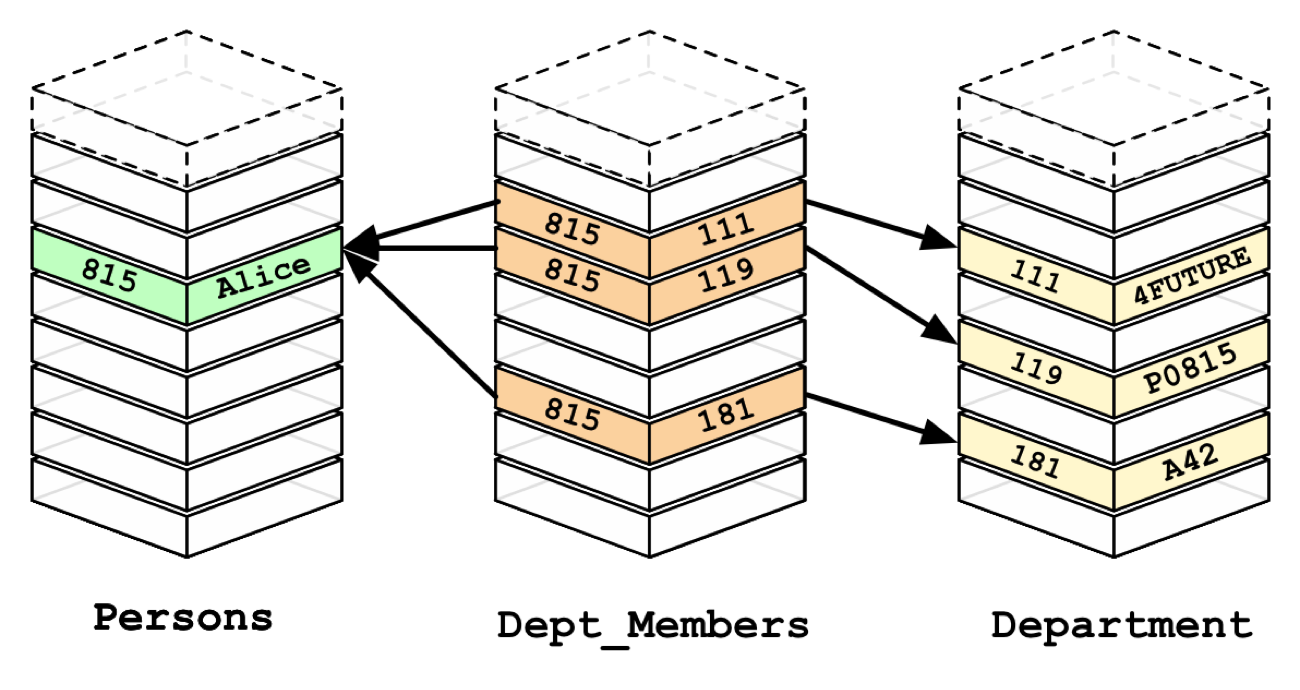
\includegraphics[width=\textwidth]{relational_databases_demo}
\end{figure}

\section{SGBD în practică}
SGBD-urile sunt folosite foarte intensiv în practica de zi cu zi atât a dezvoltatorilor soluțiilor software, atât și de către personalul \emph{data entry}, unitățile de management ale organizației, sau chiar \emph{stakeholder-ii} companiei. Majoritatea sistemelor moderne permit accesarea și vizualizarea datelor în format ușor accesibilă, cu funționalități performante de exportare pentru eventuală analitică folosind instrumente dezvoltate pentru însărcinarea propusă. 

Datele pot fi exportate în o multitudine bogată de formate pentru operațiuni diferite cu datele propuse. Exemple exacte sunt ce urmează.
\begin{itemize}
	\item  \emph{\textbf{JSON}}\footnote{\url{https://en.wikipedia.org/wiki/JSON}} pentru includerea în aplicații web sau scripturi, perfect pentru dezvoltatorii de soluții softare, ce au nevoie de un format portabil pentru integrarea datelor în \emph{\textbf{API}}-uri\footnote{\url{https://en.wikipedia.org/wiki/API}} și interfețe vizuale. 
	
	\item \emph{\textbf{XLS}}\footnote{\url{https://en.wikipedia.org/wiki/Microsoft_Excel}}, pentru includerea în aplicații de tip \emph{spreadsheet}, de tip Microsoft Excel, sau Google Sheets. 
	Este perfect potrivit pentru managerii sau contabilii unei companii pentru analiza și prognozartea informației pe baza datelor existente.
	
	\item \emph{\textbf{CSV}}\footnote{\url{https://en.wikipedia.org/wiki/Comma-separated_values}}, perfect pentru integrarea în scripturi și sisteme automatizate, de tipul instrumentariului pentru \emph{machine learning}\footnote{\url{https://en.wikipedia.org/wiki/Machine_learning}}. Este formatul perfect pentru experții domeniului \emph{data science} ce conlucrează cu dezvoltatorii pentru determinarea \textbf{pattern}-urilor în date, și prin urmare exploatarea parametrilor datelor pentru maximizarea profitabilității.
\end{itemize}

Cele mai răspândite sisteme de SGBD la momentul actual sunt următoarele.
\begin{itemize}
	\item Oracle DB
	\item MySQL
	\item PostreSQL
	\item SQLite
	\item Microsoft SQL Server
	\item IBM DB2
\end{itemize}

Ultimii ani, tot mai populare au inceput să devină SGBD bazate pe baze de date non-relaționale, așa numitul \emph{\textbf{NoSQL}}\footnote{\url{https://en.wikipedia.org/wiki/NoSQL}}. Acestea permit un nivel de flexibilitate a datelor mult mai înalt. Faptul dat este motivat prin lipsa unei structuri bine definite, ce prin folosirea sistemei \emph{\textbf{cheie-valoare}}.

Lipsa structurii induce o pierdere în performanță, condiționată prin complexititate indexării datelor, dar, beneficiul de bază este posibilitatea modificării formatării, mărimii sau a encodării datelor, \emph{\textbf{"on the fly"}}\footnote{În mișcare}, ce este foarte benefic pentru o sistemă software în creștere. De aia acest tip de baze de date a devenit foarte popular în cadrul \emph{\textbf{startup}}-urilor, deoarece această alegere tehnică le permite avansarea rapidă și modificarea datelor fără riscul de a strica datele.

Exemple ale astfel de SGBD sunt următoarele.
\begin{itemize}
	\item MongoDB
	\item Redis
	\item Amazon DynamoDB
	\item Oracle NoSQL DB
\end{itemize}

\chapter{Domeniul de studii}

\section{Scopul și obiectivele}
Crearea unui SGBD privind gestionarea datelor ce descriu schimbul de apartamente în baza locației și a prețului și generarea informației relevante pentru cumpărători în scopul creării comenzilor online.

\begin{enumerate}
	\item Gestionarea produselor de catre administratori
	
	\item În baza datelor despre produse, crearea transactiilor de catre administratori.
	
	\item Crearea rapoartelor pentru cadrele manageriale.
\end{enumerate}

\section{Descrierea domeniului}
Ultimii ani oamenii au devenit tot mai curioși și investiți în călătorii. Ca răspund la cererea crescută apar diferite concepte pentru a ușura și a ieftini acest proces. Acest produs cade exact în această categorie.

Serviciul de schimb de apartamente presupune un \textbf{exchange} de locuință de perioadă scurtă pentru cei doritori de a vedea locuri noi și de a o face mult mai ieftin decat ar fi posibil prin intermediul hotelurilor și a chiriilor. Astfel, doritorii de astfel de aventură plasează informație personală și locuința disponibilă pe platformă, iar managerii companiei, considerând descrierea și preferințele utilizatorilor propun variante de schimb la prețuri avantajoase.

\chapter{Modelarea Datelor}

\section{Modelul Conceptual}

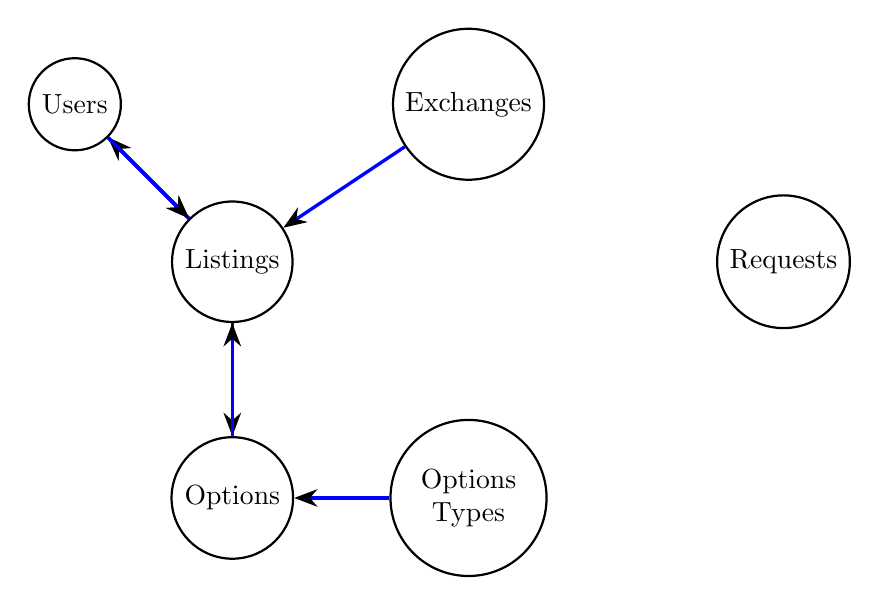
\begin{tikzpicture}
\begin{scope}[every node/.style={circle,thick,draw}]
    \node (users) at (3,4) {Users};
	\node (listings) at (5, 2) {Listings};
	\node (options) at (5, -1) {Options};
	\node[text width=1.5cm, align=center] (option_types) at (8, -1) {Options Types};
	\node (exchanges) at (8, 4) {Exchanges};
	\node (requests) at (12, 2) {Requests};

\end{scope}

\begin{scope}[>={Stealth[black]},
              every node/.style={fill=white,circle},
              every edge/.style={draw=blue,very thick}]
    \path [->] (users) edge (listings);
    \path [->] (listings) edge (users);
    	
    	\path [->] (listings) edge (users);
    	\path [->] (users) edge (listings);
    	
    	\path [->] (listings) edge (options);
    	\path [->] (options) edge (listings);
    	
    	\path [->] (option_types) edge (options);
 
    	
    	\path [->] (exchanges) edge (listings);
    	
\end{scope}
\end{tikzpicture}

\section{Modelul Logic}

Modelul logic al acestei aplicații arată în următorul mod.

\begin{figure}[H]
\center
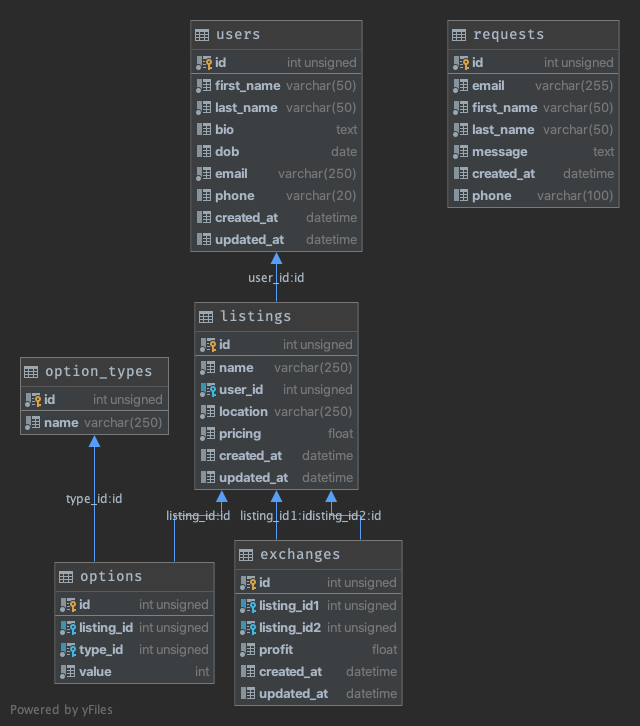
\includegraphics[width=\textwidth]{apartment_exchange}
\end{figure}

Unde cheitele aurii si albastre denotă \textbf{primary key} și \textbf{foreign key} respectiv.

\section{Descrierea datelor}

\subsection{Users}
Este tabelul în care este salvată informația despre clienții serviciului. Aici sunt salvate date despre preferințe, date de contact și cele personale pentru a utilizarea platformei.

\begin{figure}[H]
\center
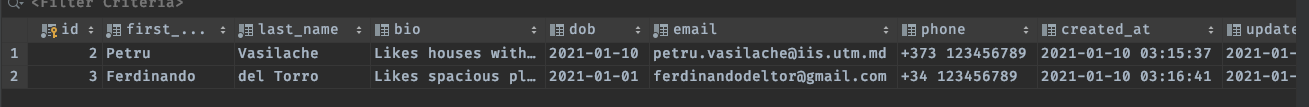
\includegraphics[width=\textwidth]{users_table}
\end{figure}

\subsection{Listings}
Este tabelul de bază ce conține datele despre toate ofertele disponibile. Acestea sunt legate cu \textbf{users} și \textbf{options} pentru a determina legăturile logice în date.

\begin{figure}[H]
\center
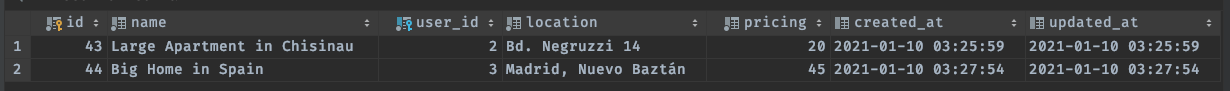
\includegraphics[width=\textwidth]{listings_table}
\end{figure}

\subsection{Options}
Este tabelul ce răspunde de indicarea relației \textbf{Many-To-Many} a ofertelor și optiunilor disponibile.

\begin{figure}[H]
\center
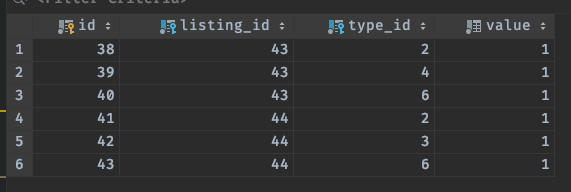
\includegraphics[width=\textwidth]{options_table}
\end{figure}


\subsection{Option Types}
Aici sunt plasate toate opțiunile disponibile.

\begin{figure}[H]
\center
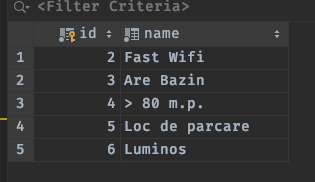
\includegraphics[width=\textwidth]{option_types_table}
\end{figure}


\subsection{Requests}
Conține datele despre cererile de pe pagina de start a aplicației. Este presupus că este punctul de primar de interacțiune cu serviciul.

\begin{figure}[H]
\center
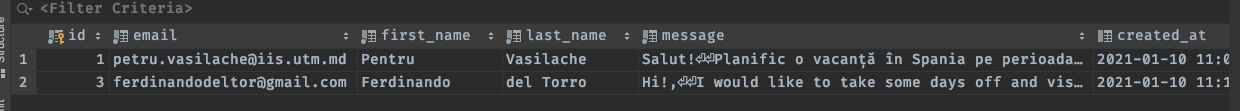
\includegraphics[width=\textwidth]{requests_table}
\end{figure}


\subsection{Exchanges}
Conține datele despre transacțiile și profitul generat de către serviuciul în cauză. Punctul primar de generare a rapoartelor.

\begin{figure}[H]
\center
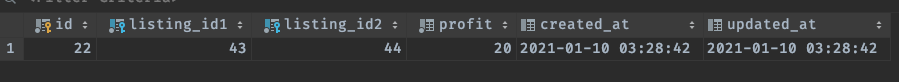
\includegraphics[width=\textwidth]{exchanges_table}
\end{figure}

\chapter{Concluzie}
Dezvoltarea acestui serviciu a fost o experiență interesantă ce a mi-a permis să privesc proiectul din dintr-o perspectivă diferită.

\end{document}